
\documentclass{beamer}
\usepackage{ctex}
\usepackage{graphicx}
\usepackage{amsmath}
\usepackage{booktabs}
\usepackage{hyperref}
\usepackage{subcaption}

% 添加参考文献支持
\bibliographystyle{alpha}

\usetheme{Madrid}
\usecolortheme{seahorse}

% 自定义块颜色
\setbeamercolor{block title}{bg=blue!30,fg=black}
\setbeamercolor{block body}{bg=blue!10,fg=black}
\setbeamercolor{exampleblock title}{bg=green!50,fg=black}
\setbeamercolor{exampleblock body}{bg=green!20,fg=black}

% 开启图表编号
\setbeamertemplate{caption}[numbered]

\title{\textbf{周报-向嘉豪(2024-11-18)}}
\author{向嘉豪}
\institute{衡阳师范学院}
\date{2024年11月18日}

\begin{document}

\begin{frame}
    \titlepage
\end{frame}

\begin{frame}
    \frametitle{摘要}
    \begin{block}{本周工作}
        本周主要对OPO(Optimization of Permutation Operation)算法进行了优化和重构:
        \begin{itemize}
            \item 重构PPO类结构提高代码可维护性
            \item 应用于AES的ShiftRow操作并进行性能测试
            \item 相比\cite{Schwabe2016}的实现,性能提升9.7\%
        \end{itemize}
    \end{block}
\end{frame}

\section{OPO算法优化}
\begin{frame}
    \frametitle{OPO算法优化}
    \begin{columns}
        \column{0.48\textwidth}
        \begin{figure}
            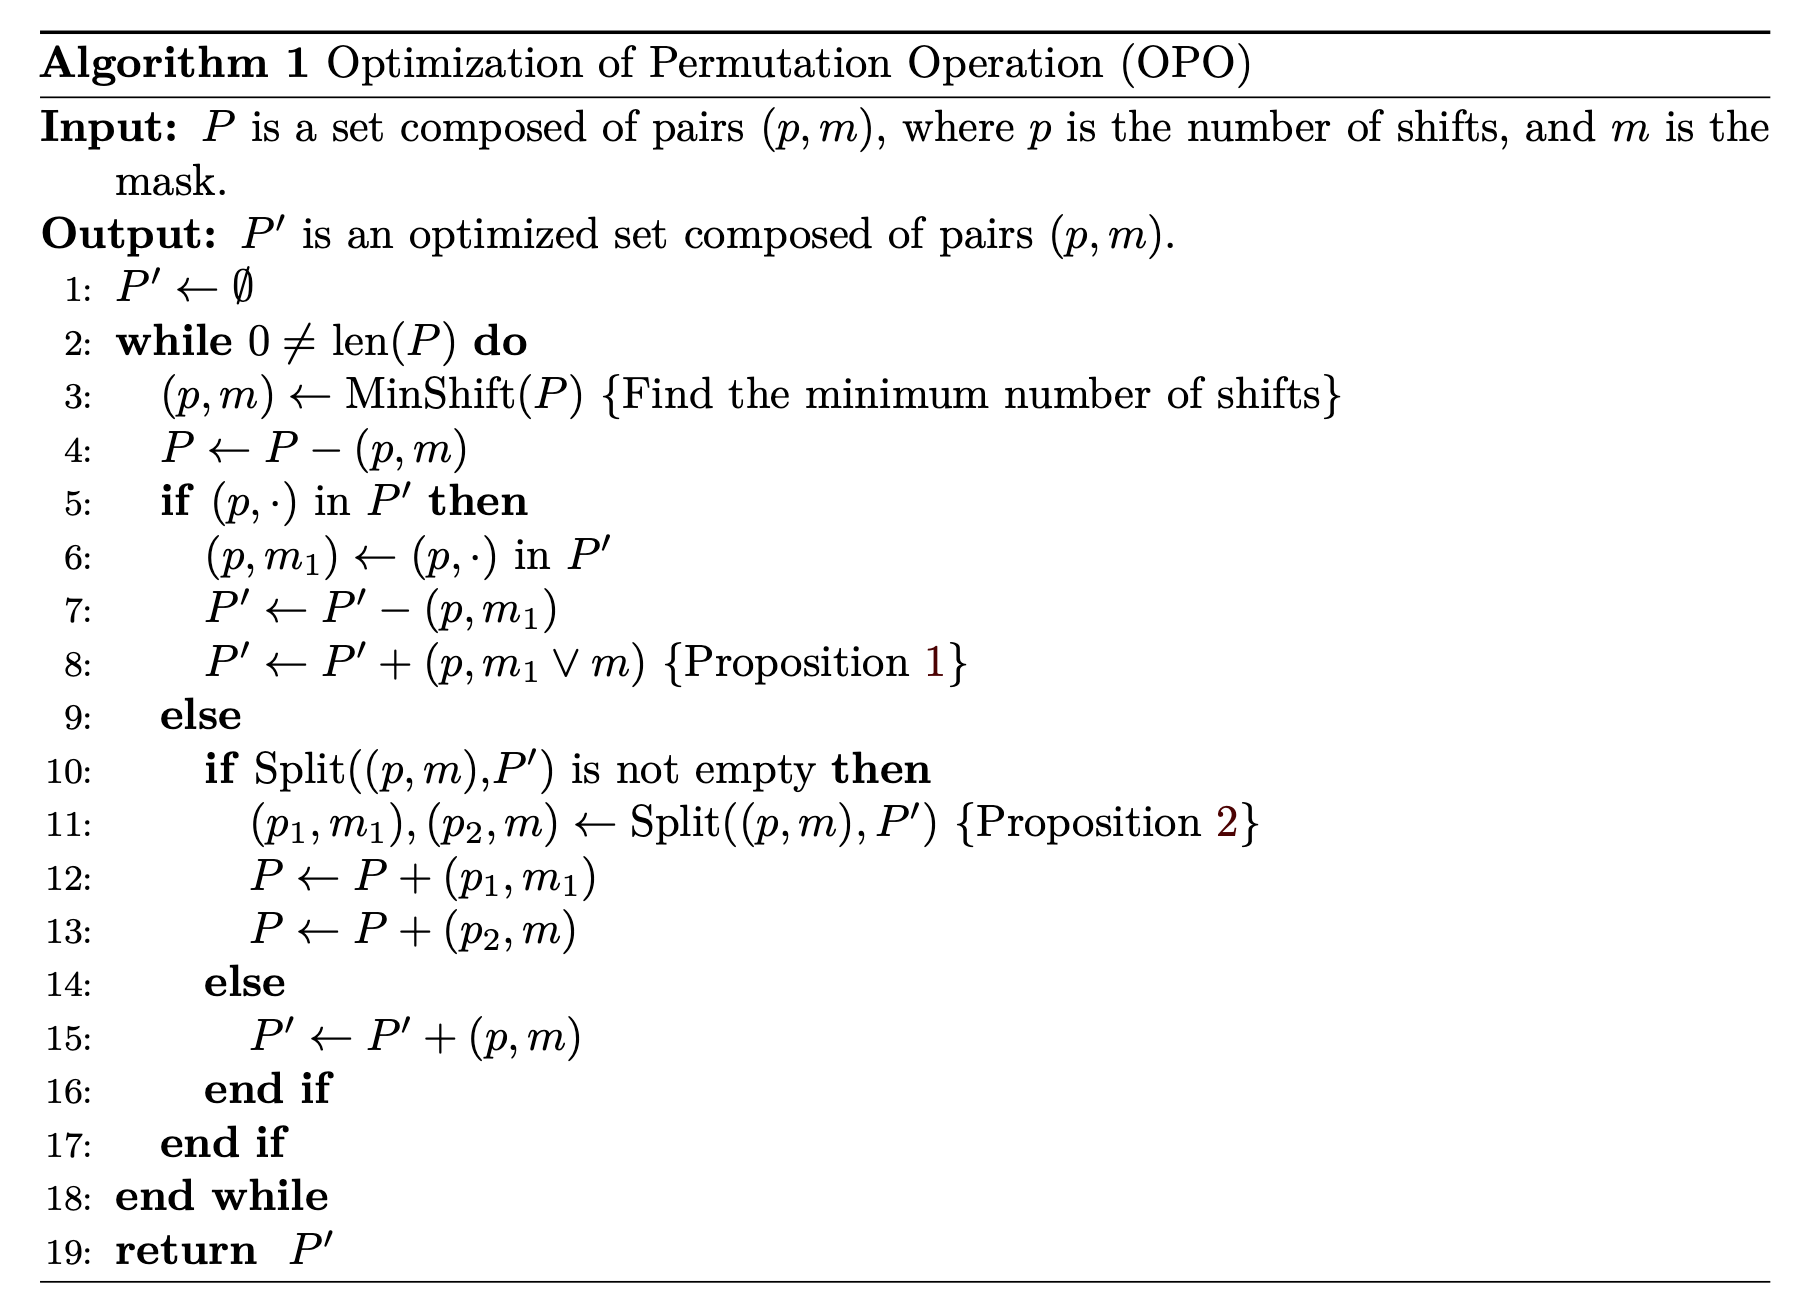
\includegraphics[width=\textwidth]{./fig/old_opo.png}
            \caption{原始OPO算法}
        \end{figure}
        
        \column{0.48\textwidth}
        \begin{figure}
            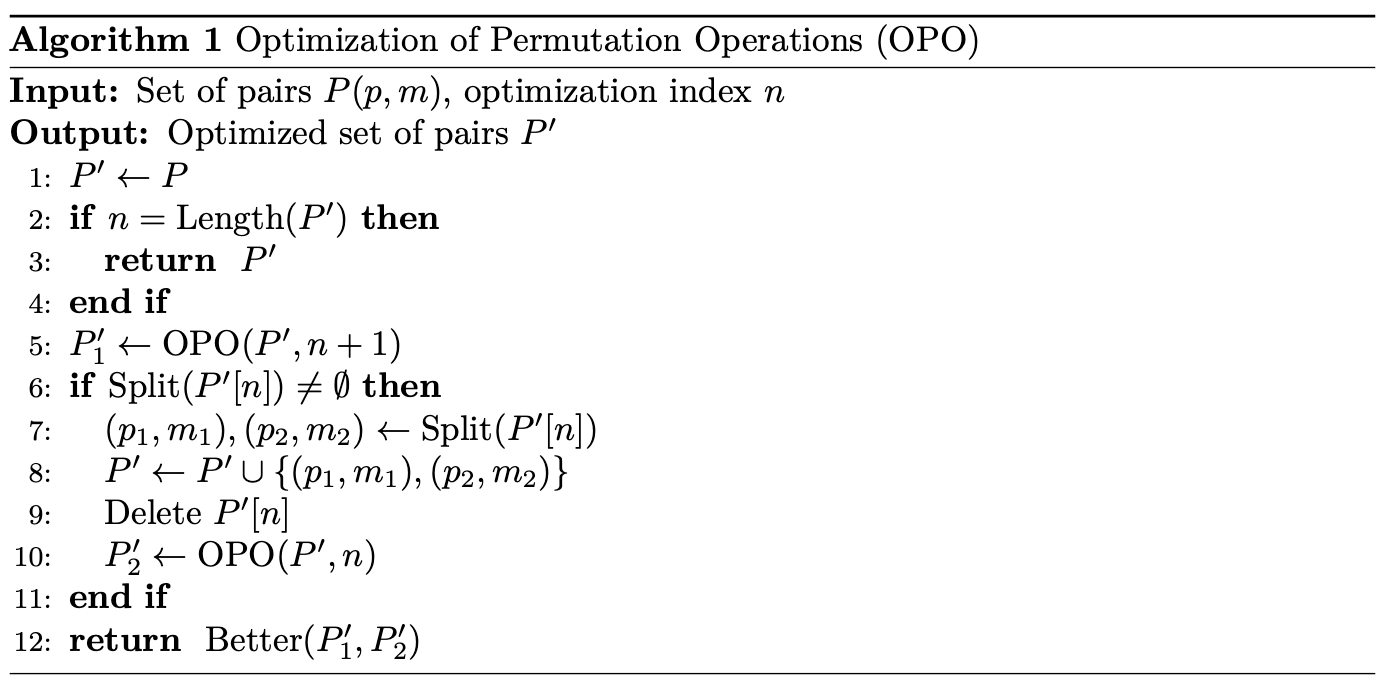
\includegraphics[width=\textwidth]{./fig/new_opo.png}
            \caption{优化后OPO算法}
        \end{figure}
    \end{columns}
\end{frame}

\begin{frame}
    \frametitle{PPO类重构}
    \begin{block}{重构目标}
        \begin{itemize}
            \item 解决手动计算中间寄存器问题
            \item 简化汇编转化过程
            \item 提高代码可维护性
        \end{itemize}
    \end{block}
    \begin{figure}
        \centering
        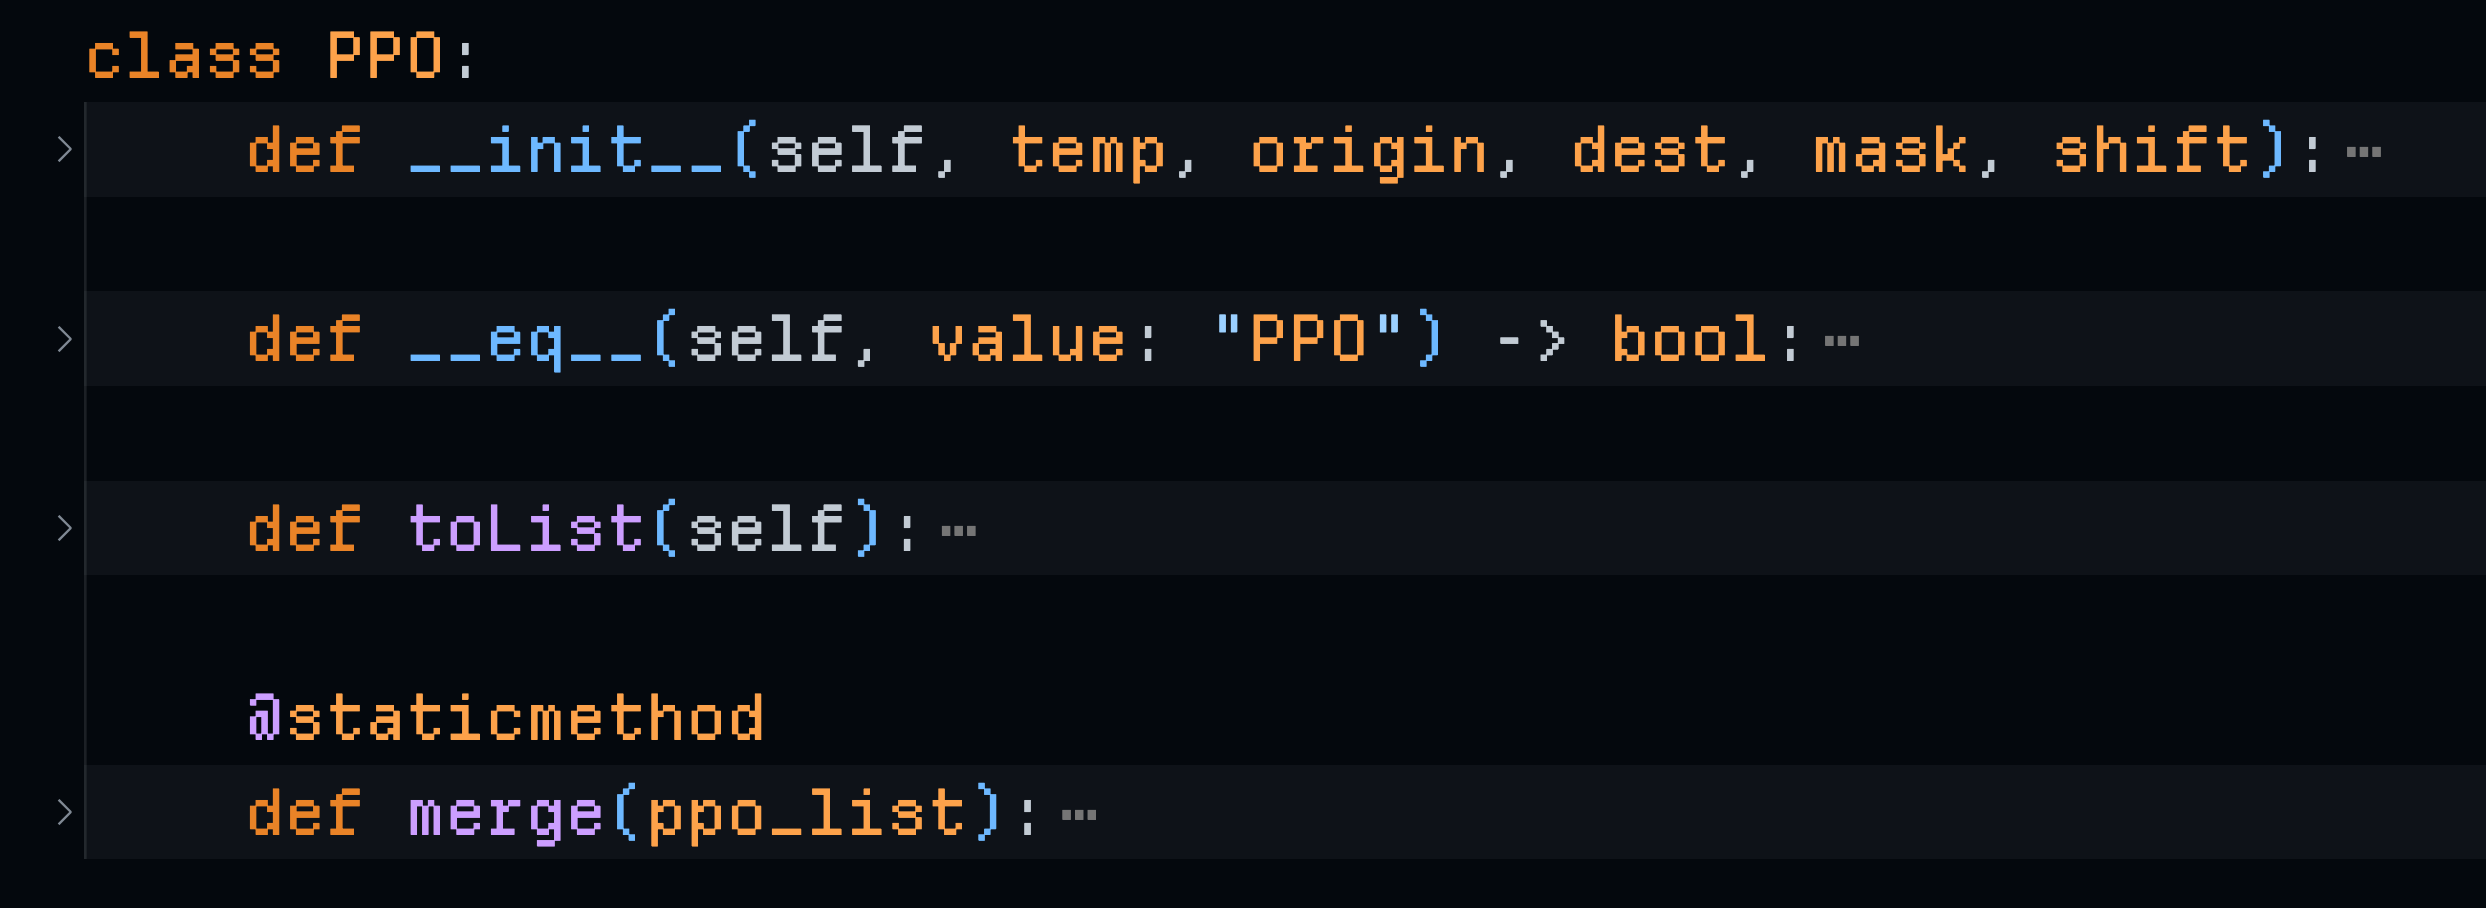
\includegraphics[width=0.7\textwidth]{./fig/ppo_class.png}
        \caption{PPO类结构}
    \end{figure}
\end{frame}

\section{OPO优化AES算法}
\begin{frame}
    \frametitle{ShiftRow优化对比}
    \begin{columns}
        \column{0.48\textwidth}
        \begin{block}{原始实现}
            操作序列:
            \begin{itemize}
                \item 7个PPO操作
                \item 较大的代码体积
            \end{itemize}
        \end{block}
        
        \column{0.48\textwidth}
        \begin{block}{优化后实现}
            操作序列:
            \begin{itemize}
                \item 5个PPO操作
                \item 更紧凑的代码
            \end{itemize}
        \end{block}
    \end{columns}
\end{frame}

\begin{frame}
    \frametitle{性能对比}
    \begin{table}
        \centering
        \caption{AES算法实现性能对比}
        \begin{tabular}{lccc}
            \toprule
            实现方案 & 优化等级 & 周期数 & Flash大小(字节) \\
            \midrule
            \cite{Schwabe2016} & O3 & 8,932 & 27,100 \\
            本文工作 & O3 & \textbf{8,068} & \textbf{25,948} \\
            \bottomrule
        \end{tabular}
    \end{table}
    
    \begin{block}{优化效果}
        \begin{itemize}
            \item 执行周期数减少9.7\%
            \item Flash内存占用减少
        \end{itemize}
    \end{block}
\end{frame}

\begin{frame}[allowframebreaks]
    \frametitle{参考文献}
    \bibliography{../../paper}
\end{frame}

\begin{frame}
    \frametitle{老师评语}
    \begin{block}{标题:Linear Layer Bitsliced Implementation Form \& Optimization Schemes \& Linear layer}
        改为 Bitsliced Implementation of Linear Layers \& Proposed Optimization Schemes \& Linear Layer Optimization
    \end{block}

    \begin{block}{全文类似的不突出不明确不清晰的很多,是不是水平就是这样,提高不了了?}
        对表述不明确的地方进行修改。
    \end{block}
    \begin{alertblock}{本周计划}
        完成论文初稿,对论文精修。
    \end{alertblock}
\end{frame}

\end{document}